\section{Prozessdiagramm des Backends}
    In diesem Kapitel werden die REST-Endpunkte des Backends und ihre Funktionsweise mithilfe von Prozessdiagrammen aufgezeigt.
    Da das Backend in Rust, einer nicht-objektorientierten Sprache, implementiert wird, ist ein Klassendiagramm nicht sinnvoll.

    Die Funktion des Backends besteht darin, verschiedene REST-Endpunkte bereitzustellen.
    Es werden hier acht Endpunkte definiert, die in drei Services (bzw. Gruppen) unterteilt werden können: \lstinline{devices}, \lstinline{datapoints} und \lstinline{targets}
    Diese Aufteilung ermöglicht eine bessere Code-Wiederverwendung innerhalb eines Services und vereinfacht außerdem die Prozessdiagramme.

    Vor Beginn der Implementierung wurden die Endpunkte in Textform formuliert.
    Zur besseren Anschaulichkeit werden hier die fertigen Endpunkte betrachtet, die in Abbildung~\ref{fig:swagger-endpoints} basierend auf der generierten OpenAPI-Dokumentaion mithilfe von SwaggerUI dargestellt sind
    \footnote{Vollständige Dokumentation inkl. Datentypen ist unter https://se-backend.fly.dev/swagger-ui einsehbar}.
    Im Folgenden wird für jeden Service ein Prozessdiagramm vorgestellt.

    \begin{figure}[H]
        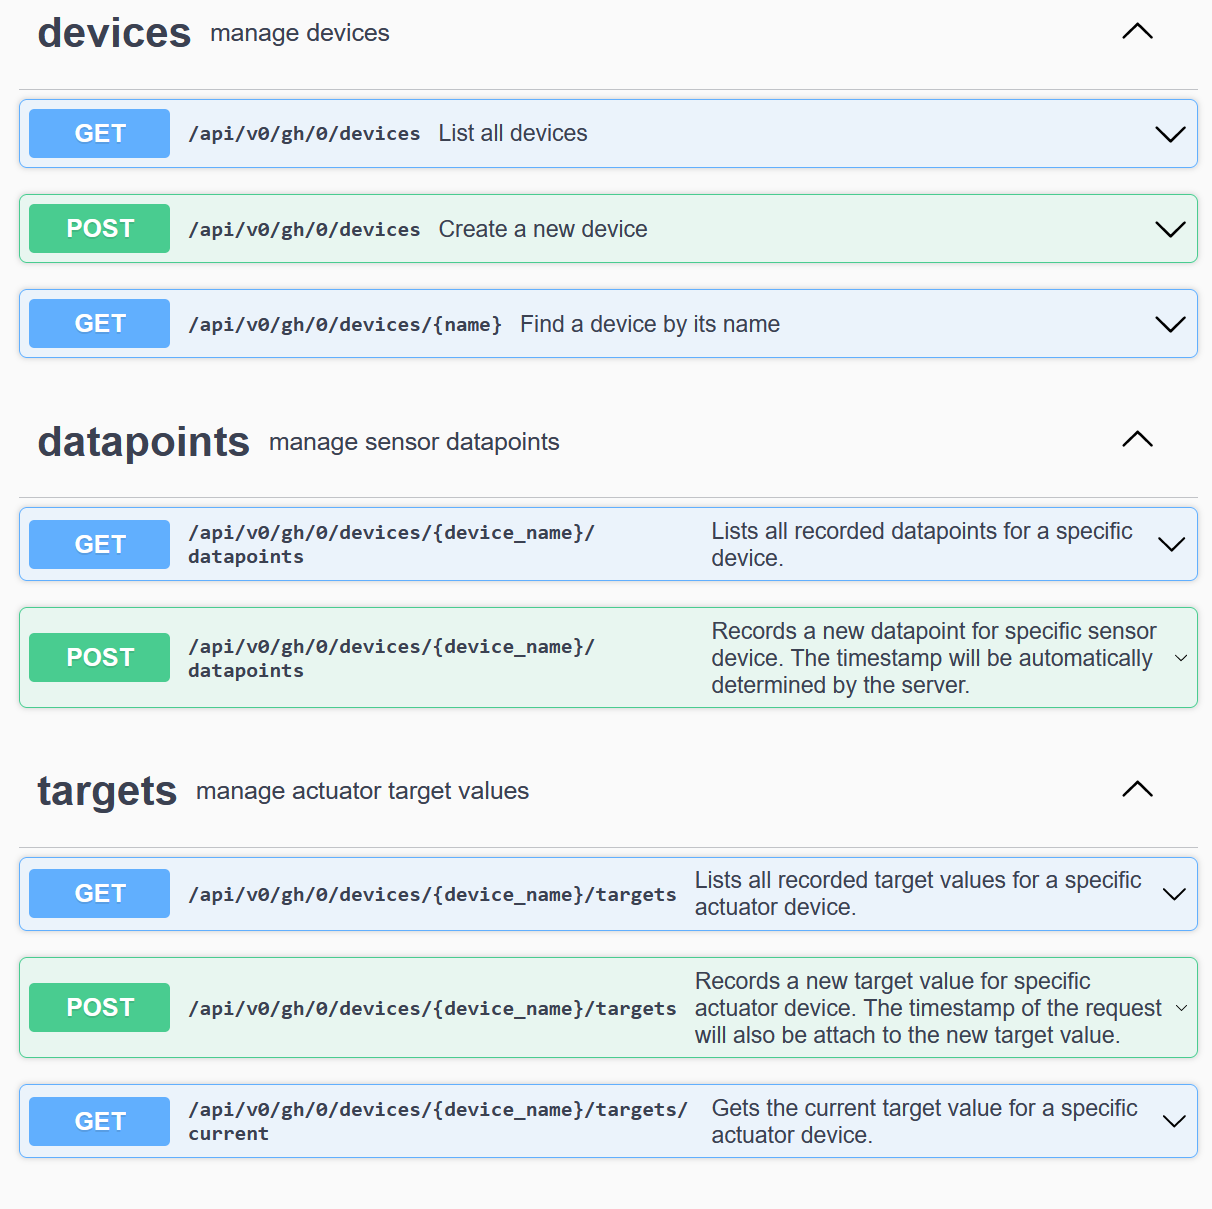
\includegraphics[width=0.95\linewidth]{images/swagger-endpoints.png}
        \centering
        \caption{REST-Endpunkte (Rendering der OpenAPI-Dokumentaion durch SwaggerUI)}
        \label{fig:swagger-endpoints}
    \end{figure}


    \subsection{devices-Service}
        Der devices-Service umfasst mehrere Endpunkte zum Erstellen oder Abfragen von Devices, also Sensoren oder Aktoren der Hardware.
        In Abbildung~\ref{fig:backend-service-devices} sind die nötigen Prozesse dargestellt.

        Zuerst wird bei den Endpunkten (in blau) überprüft, ob die übergebenen JSON-Felder valide sind.
        Falls dies nicht der Fall ist, wird ein entsprechender Fehlerstatuscode (hier: 400 Bad Request) zurückgegeben.
        Diese Überprüfung wird in den folgenden beiden Unterkapiteln zu den anderen Services weggelassen, ist aber dennoch überall nötig, wo es JSON-Parameter gibt.

        Im Anschluss wird bei allen drei Endpunkten eine Anfrage an die Datenbank gemacht und dann entweder das Ergebnis oder ein Fehlerstatuscode zurückgegeben.

        \begin{figure}[H]
            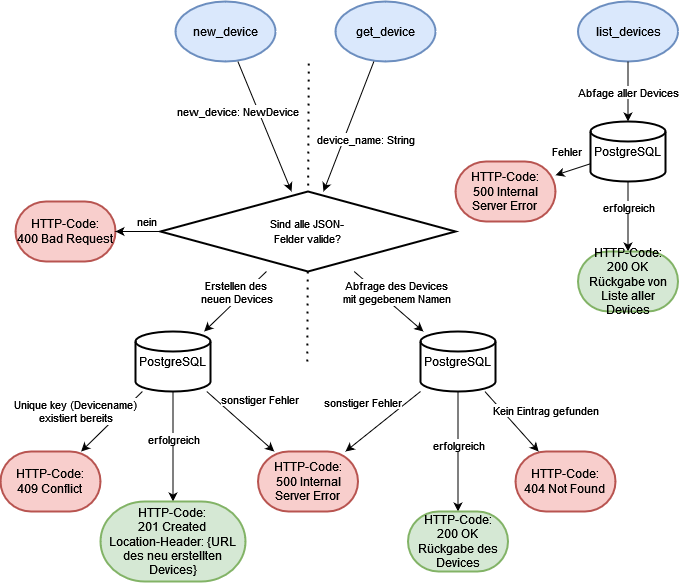
\includegraphics[width=0.95\linewidth]{images/prozessdiagramm_backend_devices.drawio.png}
            \centering
            \caption{Prozessdiagram der Endpunkte im devices-Service}
            \label{fig:backend-service-devices}
        \end{figure}

    \subsection{datapoints-Service}
        Der datapoints-Service verwaltet die Datenpunkte eines Sensor-Devices.
        Hier sind zwei Endpunkte zum Erstellen eines neuen Sensor-Datenpunktes und zum Abfragen aller Datenpunkte nötig.
        Beide haben gemeinsam, dass das angefrage Device vom Typ Sensor sein muss, weshalb im Prozessdiagramm in Abbildung~\ref{fig:backend-service-datapoints} die oberen Prozesse zusammengefasst sind.
        Nach der Device-Typ Überprüfung wird in beiden Fällen eine weitere Anfrage an die Datenbank gemacht und das Ergebnis oder ein Fehlerstatuscode zurückgegeben.
        \begin{figure}[H]
            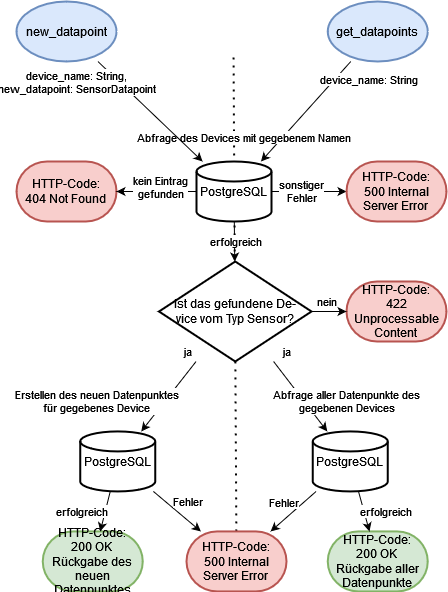
\includegraphics[width=0.7\linewidth]{images/prozessdiagramm_backend_datapoints.drawio.png}
            \centering
            \caption{Prozessdiagram der Endpunkte im datapoints-Service}
            \label{fig:backend-service-datapoints}
        \end{figure}

    \subsection{targets-Service}
        Der targets-Service ist für die Endpunkte zuständig, welche die Zielwerte (TargetValues) von Actuator-Devices setzen und abfragen.
        Es werden wie bei den Sensor-Datenpunkten zwei Endpunkte zum Erstellen und Abfragen aller Targets und zusätzlich ein Endpunkt zum Abfragen des aktuellsten Zielwertes angeboten
        \footnote{ Obwohl die Hardware nur begrenzte Ressourcen zur Verfügung hat, kann sie so nur den aktuellsten Wert abfragen. Außerdem könnte so das Backend in der Zukunft mit Logik wie dem Auflösen eines Zeitplans erweitert werden, ohne dass die Hardware angepasst werden muss. }.

        Auch hier erfolgt zuerst eine gemeinsame Überprüfung, ob das angefrage Device ein Aktuator ist.
        Daraufhin wird je nach Endpunkt eine Datenbank-Anfrage getätigt und das Ergebnis oder ein Fehlerstatuscode zurückgegeben.

        \begin{figure}[H]
            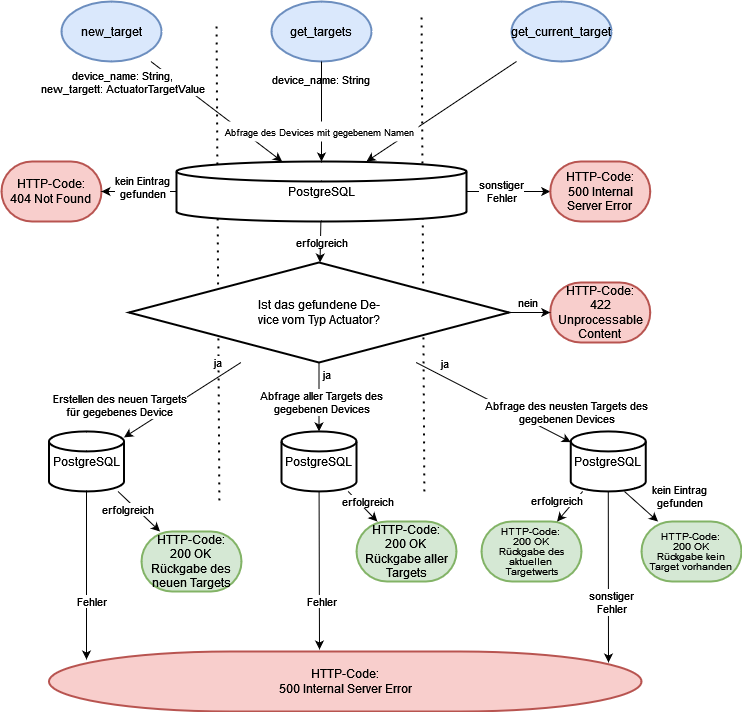
\includegraphics[width=1.05\linewidth]{images/prozessdiagramm_backend_targets.drawio.png}
            \centering
            \caption{Prozessdiagram der Endpunkte im targets-Service}
            \label{fig:backend-service-targets}
        \end{figure}

\pagebreak
